\chapter{Background}
\label{chap:background}

\section{Definitions and vocabulary}
\label{sec:background_definitions}

\subsection*{Identity}
A set of attributes that identifies an entity~\cite{Weik2001}. An entity can be a system, process or individual, but identity in this paper will exclusively reference a persons identity if not explicitly stated otherwise. 
\subsection*{Identity Owner}
The owner of the digital identity, also known as the user.

\subsection*{Identity Provider}
An entity that verifies and signs attributes associated with an identity to provide a certain level of trust in the validity of the information. This could be governmental bodies, banks and other entities that service providers trust.

\subsection*{Service Provider}
An entity that provide some sort of service, and in this context is reliant on a knowing some information relating to the identity of the user. An example of this could be a gambling website ensuring their users are over 18 years of age.

\subsection*{Claims}
Attributes a user or identity owner presents to a service provider 

\section{Traditional Identity Systems}
The most common user management in online services today is still the traditional localized register of users where the user has to sign up with their information directly on the website, and this poses several challenges for both the user and the service provider. For the user, this often forces them to either use the same password on several services, or manage a increasingly large number of passwords. The number of online services an average person uses today, having different passwords for each is a daunting task, often eliminating this option. If the user uses the same password everywhere, chances are one of those services uses bad practices and the password is leaked and the adversary can access all the users accounts using the same password. For the service provider, the users are trusting them with personal information that they have to manage and protect responsibly.

The second most used method is federated identities, where the user trusts one identity provider and registers with them. The user can then log in to several services using the same account. Most known applications of this is seen on websites that has the option "Sign in with Facebook/Google". This also poses some challenges; the user rely on one provider to store and protect their data, and also facilitating for tracking and big data gathering as that provider will get information on what services the user is accessing when.

\section{Distributed Ledgers}
\label{sec:background_dlt}
\subsection{Blockchain}
Bitcoin was the first application of a blockchain, and is based on a proof-of-work system to represent a majority decision. The miners collect pending transactions in the network and form potential blocks, illustrated in Figure \ref{fig:blockchain}, and then, hash the contents of this block with an variable nonce to meet a certain criteria~\cite{bitcoin2008}. For Bitcoin this criteria is that the hash must begin with a certain number of zeros, and this number of zeros can be increased or decreased to compensate for variable computational power in the network~\cite{bitcoin2008}. The complexity is varied to maintain around one block per 10 minutes, but the nature of the psudorandomization of hashing algorithms it can be solved in seconds, but it can also take in excess of 20 minutes~\cite{blockchain_info}. As long as the majority of computational power is controlled by nodes not trying to attack the network, the blockchain serves as a ledger of witnessed transactions with proved ownership.

\begin{figure}[ht]
    \centering
    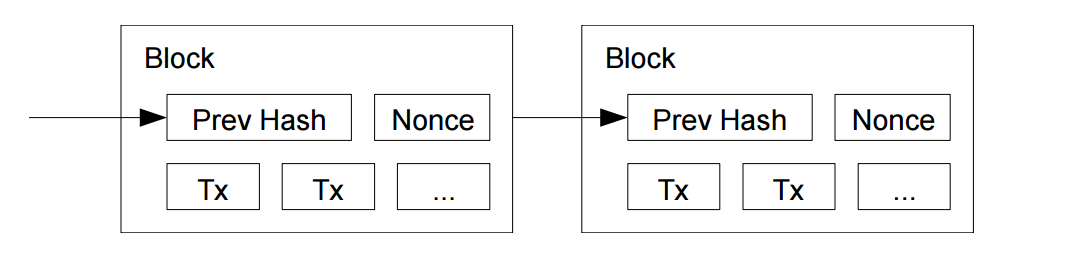
\includegraphics[width=1\textwidth]{blockchain}
    \caption{Visualization of blockchain \cite{bitcoin2008}}
    \label{fig:blockchain}
\end{figure}

The growing success of cryptocurrency, or crypto tokens, the incentive for miners has increased with the price. \cite{VRANKEN20171} estimates the total power consumption to be between 100 and 500 MW, the equivalent of a small nation state, and the inefficiency of the Proof-of-Work (PoW) has made Proof-of-Stake (PoS) look like a strong candidate. In the later years, several PoS currencies has been proposed and launched~\cite{Li2017,nxt_whitepaper,blackcoin_pos} but have yet to achieve large market adoption. The PoS scheme maintain consensus in the network based on the nodes stake, and the consensus is fast and uses negligible resources. PoS implementations sill suffer from some major security concerns, and proposed attacks like~\textit{nothing at stake} and \textit{long-range attacks} is probably holding the adoption back~\cite{Li2017}.

\subsection{Directed Acyclic Graphs }

Directed Acyclic Graph (DAC), here based on the tangle implementation in IOTA~\cite{IOTA_Whitepaper}, provides some very beneficial properties of a Distributed Ledger for Identity Management. The transactions are instant and without traditional fees, and are designed to scale infinitely. The tangle is based on a Directed Acyclic Graph (DAG) rather than a traditional chain of blocks, where each transaction is stored separately in the graph, illustrated in Figure~\ref{fig:tangle}. To make a transaction on the IOTA network, the issuing party must approve two previous transactions, thus strengthening the security of the network. IOTA is still in development, and are still working out some fundamental issues in their implementation. The IOTA foundation recently launched their data market place~\cite{IOTA_Marketplace}, and with this a series of well known industry leaders like Microsoft, Fujitsu, Accenture, and NTNU will participate in the two month beta ending in January/February 2018. IOTA aims to be the backbone of Machine-to-machine and IOT economy.

\begin{figure}[ht]
    \centering
    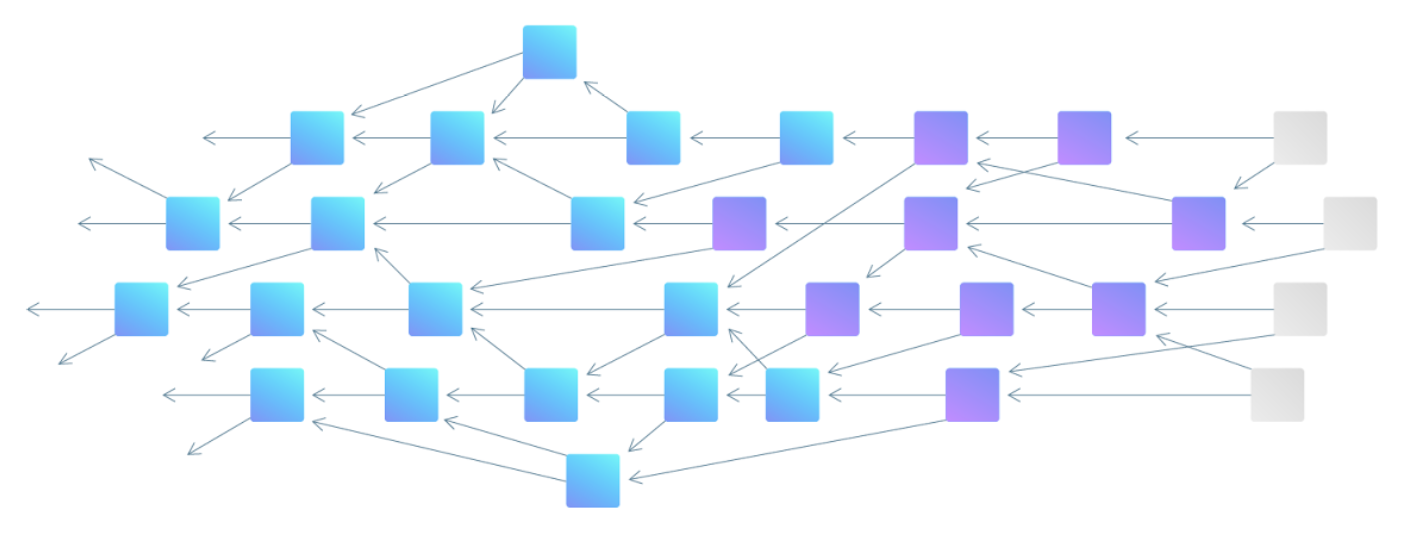
\includegraphics[width=1\textwidth]{tangle}
    \caption{Visualization of the tangle \cite{IOTA_Whitepaper}}
    \label{fig:tangle}
\end{figure}
The web of trust is a public-key authentication system originally built on PGP. A user can build confidence in their identity by having other users sign their public key~\cite{Azouvi2017}. In an identity management system where we distinguish between Users and Service Providers, we can build on this idea. We can look at a scenario where a User has their identity verified and signed by visiting the governmental department issuing passports for their citizens. If the user wants proof that they also have a drivers license, and the issuing body (DMV, Statens Vegvesen, e.g.) trusts that department, they can link a drivers license to that identity based on the verified identity already in the ledger. This opens up for possibilities where the User can visit a small number of Identity Providers and establish a base identity, and then build upon that over the internet.

\subsection{Gossip Protocol}
https://link.springer.com/chapter/10.1007/978-3-319-14977-6\_28

\section{Self-Sovereign Identity (SSI)}
When Self-Sovereign Identity (SSI) is used as a term within this paper, if references a model of identity management that ensures that the user fully owns and controls their own data. This also includes who has access to the attributes and the possibility to add, delete or revoke these attributes at their own discretion. To assure the privacy required by a SSI-model, the attributes must be stored and processed in a secure manner, and segregation of attributes such that anyone other than the owner can connect the different attributes to the identity. The identity must be maintained and stored without a federation or third party control, and is therefor reliant on a distributed and truly decentralized system.

Even though EGIZ Whitepaper on Self-Sovereign Identity~\cite{ssi} is not technically correct on all the blockchain details, they have a good definition on Self-Sovereign Identity that I have used to define SSI in the context of this thesis. This whitepaper also states that a requirement for a self-sovereign identity model is that access to the information is logged. This is a trade-off between privacy and security and is discussed further in INSERT CHAPTER HERE. 

\section{Available Self-Sovereign Identity Systems}
\label{sec:ssi_systems}
\subsection{Sovrin}
The Sovrin Foundation have set out on a mission to standardize and create an infrastructure for Self-Sovereign identities, using blockchain as storage for Distributed Identities such that anyone can issue or verify it~\cite{sovrin}. The Sovrin blockchain has been designed only for identity, and is taking steps to move the digital trust away from centralized CAs to a web of trust model. The Soverin SSI model is not dependent on any particular distributed ledger, but can work with any blockchain that meets the fundamental principles. Sovrin has implemented their identity system in a specific instantiation of Hyperledger's Indy project.
\\\\
https://sovrin.org/wp-content/uploads/Sovrin-Protocol-and-Token-White-Paper.pdf
\\\\ https://sovrin.org/wp-content/uploads/2017/04/The-Technical-Foundations-of-Sovrin.pdf
\\\\
https://www.evernym.com/solution/
https://www.evernym.com/

\subsection{uPort}
https://whitepaper.uport.me/uPort\_whitepaper\_DRAFT20170221.pdf


\subsection{Civic}
https://www.civic.com/

\subsection{Comparison}
\begin{table}[ht]
\begin{center}
\begin{tabular}{|l|c|c|c|}
\hline
 & Sovrin & uPort & Civic \\
\hline
Minable & No & Yes & Yes  \\
Attribute Segregation & Yes & Yes & Yes \\
Storage & On-Chain & Off-Chain & On-Device \\
Smart Contracts & No & Yes & Yes \\
Key Management & DPKI & DPKI & Ethereum Addresses \\
Verification & Permissioned & Permissionless & Permissionless  \\
\hline
\end{tabular}
\caption[Comparison of SSI Systems]{Tabular comparison of Self-Sovereign Identity Systems currently available}
\label{tbl:SSIS}
\end{center}
\end{table}